\section{Qualit\'e Brouillon}

Plusieurs options peuvent être désactivées ou accordées afin d'obtenir une vitesse de génération de code G plus rapide et des temps d'impression plus courts.

\subsection{Print Settings \textgreater Layers and perimeters \textgreater Quality}

\begin{figure}[H]
\centering
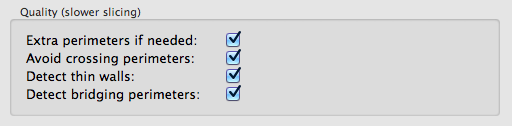
\includegraphics[keepaspectratio=true,width=1\textwidth]{advanced/draft_quality_options.png}
\caption{Option de Qualit\'e}
\label{fig:draft_quality}
\end{figure}

Ces options fournissent des objets plus agréables et plus propres, mais nécessitent plus de temps CPU. Elles peuvent être désactivées pour les impressions en mode broullion.

\begin{itemize}
\item \texttt{Extra perimeters if needed} Cette fonctionnalité vérifie si l'ajout de paramètres à des couches en pente aiderait à masquer le remplissage interne, ce qui rend l'objet plus agréable.
\item \texttt{Avoid crossing perimeters:} Cette fonctionnalité mélange les déplacements afin que la buse reste à l'intérieur ou à l'extérieur de l'objet chaque fois que possible, ce qui réduit le nombre de fois qu'elle traverse les périmètres et déclenche une rétraction. Cela empêche la mise en chaîne mais nécessite beaucoup de temps CPU pendant l'exportation de code G car des algorithmes complexes de planification de mouvement sont utilisés pour chaque couche unique.
\item \texttt{Detect thin walls:} Cette fonctionnalité vérifie les collisions entre les périmètres. Il garantit que l'imprimante n'essaie pas d'extruder des chemins trop rapprochés et utilise l'algorithme de l'axe médian pour transformer des parois minces en extrusions à simple passage.
\item \texttt{Detect bridging perimeters:} Cette caractéristique détecte les portions de pont / surplomb des périmètres et leur applique le débit / vitesse de pont.
\end{itemize}

\subsection{Print Settings \textgreater Infill}

Lesmotifs de remplissage \textit{Hilbert Curve}, \textit{Archimedean Chords} et \textit{Octagram Spiral} sont généralement beaucoup plus lents. Vous pourriez vouloir les éviter dans vos tirages de qualité d'ébauche si vous vous souciez de la vitesse de découpage.

\subsection{Print Settings \textgreater Advanced \textgreater Resolution}

Par défaut, Slic3r ne simplifie pas la géométrie d'entrée et rendra tous les détails dans le G-code de sortie pour une précision maximale. Cependant, les modèles à haute résolution portent souvent plus de résolution que l'imprimante est capable d'imprimer, de sorte qu'ils peuvent être simplifiés, surtout lorsque vous voulez un découpage plus rapide. Vous pouvez définir l'option de résolution à quelque chose comme 0,05 mm ou même 0,1 mm pour vos tirages de qualité de tirage.

\subsection{Print settings \textgreater Advanced \textgreater Threads}

(Cet indice s'applique à tous les types d'impressions, pas seulement à la qualité du trait.) De nombreux algorithmes dans Slic3r supportent la parallélisation en utilisant plusieurs threads. Vous devez définir cette option sur le nombre de processeurs ou de noyaux de votre ordinateur.
